\chapter{VARIATIONS OF GAN}
\begin{onehalfspace}
    Ian Goodfellow and his collaborators introduced GANs in 2014. Since then 
    they were studied extensively by researchers around the globe. As a result, 
    more than 450 different types of GANs have been proposed by 
    researchers \cite{gan_list}. 

    The idea of GAN has been applied extensively in many domains, which 
    resulted in a variety of interesting deep learning models. GANs have been 
    used for "image to image" translation. Image-to-image translation is a 
    class of vision and graphics problems where the goal is to learn the 
    mapping between an input image and an output image using a training set of 
    aligned image pairs. CycleGAN \cite{CycleGAN2017} transfers pictures from 
    one domain to another. 
    
    It is also capable of performing artistic style transfer, adding bokeh 
    effect to phone camera photos, creating outline maps from satellite images 
    or convert zebras to horses and vice versa, to list a few 
    \cite{cycleganprojectpage}. Figure \ref{fig:cyclegan} shows CycleGAN 
    transforming Monet paintings to landscape images.

    \begin{figure}[h]
        \centering
        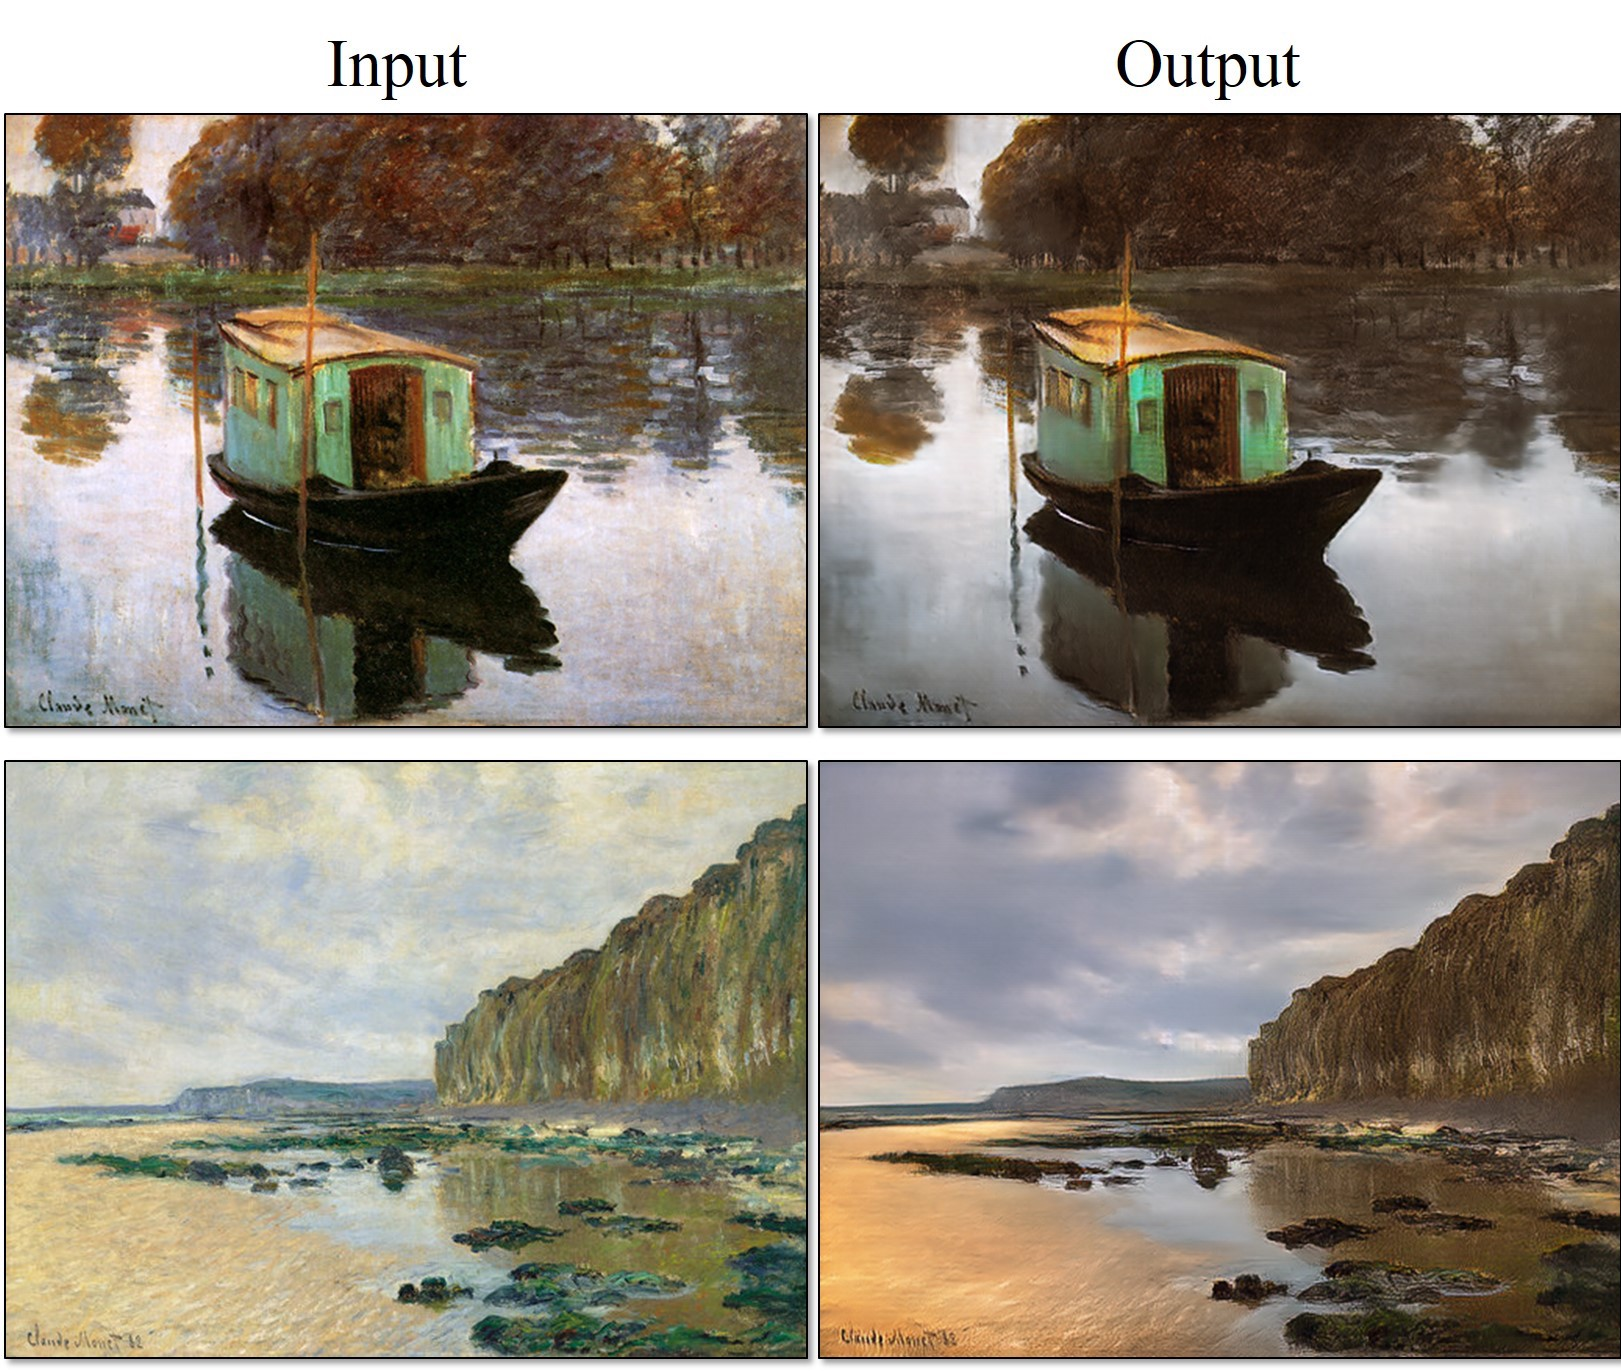
\includegraphics[width=0.6\linewidth]{images/painting2photo.jpg}
        \caption{CycleGAN mapping Monet paintings (input) to landscape photographs (output)
        \cite{cycleganprojectpage}}
        \label{fig:cyclegan}
    \end{figure} 

    In the following sections, the report gives a brief overview of 
    some of the most prominent applications of GAN. Section 3.1 discusses 
    text-to-image synthesis using GAN, and section 3.2 describes a GAN for 
    image super resolution.

    \section{Generative Adversarial Text to Image Synthesis}
    Advancements in Recurrent Neural Networks has enabled the creation of 
    powerful architectures to learn discriminative text feature representations. 
    Meanwhile, Deep Convolutional GANs (DCGANs) have begun to create highly 
    realistic images belonging to specific categories. Generative Adversarial 
    Text to Image Synthesis \cite{texttoimagegan} bridges these advancements in 
    text and image modelling. 
    The architecture aims to transform human descriptions of images in single 
    sentences directly into image pixels (See figure \ref{fig:stockgan}).

    Text to image synthesis is a challenging problem consisting of two parts: 
    first, learn a text feature representation that captures the essential 
    visual details and second, synthesise an image that seems real to a human. 
    Fortunately, deep learning has made significant progress in both areas. 
    However, one difficult issue not solved by deep learning is that there 
    exist many plausible combinations of pixels that correctly illustrate the 
    definition. By conditioning both the discriminator and generator on side 
    information, we can naturally model this phenomenon as the discriminator 
    acts as a smart adaptive loss function.

    \begin{figure}[h]
        \centering
        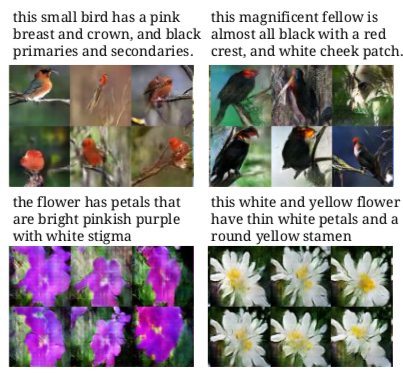
\includegraphics[width=0.6\linewidth]{images/texttoimage.png}
        \caption{Images generated by the GAN along with the text description 
        used to generate them \cite{texttoimagegan}}
        \label{fig:stockgan}
    \end{figure} 

    \section{SRGAN}
    Estimation of the high-resolution image from its low-resolution counterpart 
    is called super-resolution (SR). The goal of supervised SR algorithms is to 
    reduce the Mean Squared Error (MSE) between the generated high-resolution 
    image and the target image. Minimizing  MSE also maximises Peak Signal to 
    Noise Ratio (PSNR). MSE and PSNR are the most common methods used to judge 
    SR algorithms. 
    As MSE and PSNR are evaluated on pixel-wise differences, they fail to 
    identify perceptually relevant differences such as high texture detail. 

    SRGAN \cite{srgan} employ dee residual network with skip-connection. It defines a novel 
    perceptual loss using high-level feature maps of VGG network, and a 
    discriminator that favours solutions perceptually hard to differentiate 
    from high-resolution reference images. As figure \ref{fig:srganimage},
    suggests, the image produced by SRGAN is able to produce sharper images when 
    compared to other networks.

    \begin{figure}[h]
        \centering
        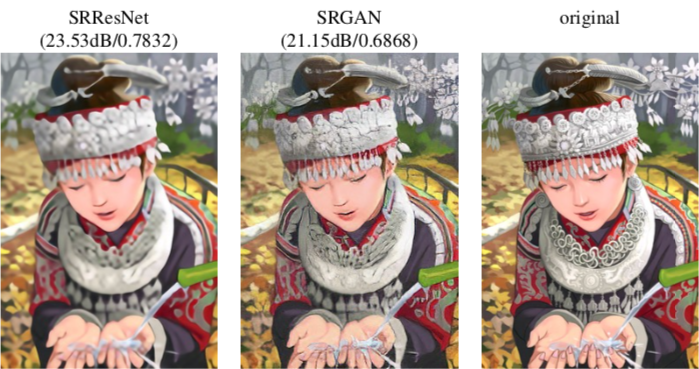
\includegraphics[width=0.9\linewidth]{images/srgan.png}
        \caption{From left to right: bicubic interpolation, deep residual 
        network optimized for MSE, deep residual generative adversarial network 
        optimized for a loss more sensitive to human perception, original 
        HR image. Corresponding PSNR and SSIM are shown in brackets. 
        (4 x upscaling) \cite{srgan}}
        \label{fig:srganimage}
    \end{figure} 

    In chapter \ref{chapter:vae}, the report describes another prominent 
    approach to generative modelling, the variational autoencoders.
    
\end{onehalfspace}